\documentclass{article}

% Encoding and Geometry
\usepackage[utf8]{inputenc}
\usepackage[a4paper, margin=1in]{geometry} % Standard 1-inch margins for better layout
\usepackage{parskip}

% Math Packages
\usepackage{amsmath, amsfonts, mathtools}

% Graphics and Figures
\usepackage{graphicx}
\usepackage{caption}
\usepackage{subcaption}
\usepackage{multirow}
\usepackage{tikz}
\usetikzlibrary{positioning} % Ensures compatibility with Overleaf

% Hyperlinks
\usepackage[colorlinks=true, linkcolor=blue, urlcolor=blue]{hyperref} % Load last to avoid conflicts

% Floating Objects Placement
\usepackage[section]{placeins} 

% Bibliography
\usepackage[
    backend=biber,
    style=alphabetic,
    sorting=ynt
]{biblatex}
\addbibresource{references.bib}

% Title Information
\title{EulerSwap White Paper}
\author{Euler Labs}
\date{February 2025}

\begin{document}

\maketitle

\begin{abstract}    
EulerSwap is an Automated Market Maker (AMM) that improves capital efficiency using Euler lending vaults. Unlike traditional AMMs that fragment liquidity across multiple pools, EulerSwap allows a single, cross-collateralised vault to support multiple asset pairs at once. Through the Ethereum Vault Connector (EVC), market makers can borrow the out token of a swap using the in token as collateral, unlocking deep liquidity. This model enables up to 40x the liquidity depth of traditional AMMs by making idle assets more efficient. At its core, EulerSwap uses a flexible AMM curve to optimise swap pricing, ensuring deep liquidity while maintaining market balance. By combining on-demand just-in-time liquidity, shared liquidity across pools, and customisable AMM mechanics, EulerSwap reduces inefficiencies in liquidity provision, offering deeper markets, lower costs, and greater control for liquidity providers.
\end{abstract}

\section{Introduction}

EulerSwap is a novel Automated Market Maker (AMM) that increases capital efficiency and liquidity depth beyond traditional AMMs. By leveraging Euler lending vaults and just-in-time liquidity provisioning, EulerSwap enables market makers to service significantly larger swaps while reducing the need for fragmented liquidity pools.

This is achieved through a combination of advanced liquidity mechanisms and customisable AMM curves. Unlike conventional AMMs that require separate liquidity pools for each asset pair, EulerSwap utilises a single, cross-collateralised vault to support multiple asset pairs simultaneously. When a user initiates a swap, EulerSwap borrows the required out token against the in token as collateral using the Ethereum Vault Connector (EVC), dynamically scaling liquidity without requiring large static deposits.

This liquidity-sharing model increases capital efficiency, allowing EulerSwap to achieve up to 40x the liquidity depth of traditional AMMs. The integration of \href{https://docs.euler.finance/developers/evc/keyConcepts?_highlight=operator#batch-operations}{check deferrals} and \href{https://docs.euler.finance/developers/evc/keyConcepts?_highlight=operator#operators}{operator features} further enables market makers to automate liquidity provisioning and optimise capital usage.

Beyond individual swap accounts, EulerSwap enhances liquidity further by allowing multiple swap accounts to operate within the same lending vault. This modular design ensures that idle liquidity is repurposed efficiently across multiple trading pairs. Much like Curve’s 3pool, but generalised to any number of asset pairings, a USDC vault could provide deep liquidity for 10+ correlated assets without requiring separate liquidity pools for each.

EulerSwap’s exchange rates are governed by a highly customisable AMM curve (illustrated in Figure \ref{fig:fig1}), which dynamically adjusts incentives to maintain market balance. Unlike traditional AMMs that use constant-sum or constant-product formulas, EulerSwap’s curve allows for asymmetric liquidity deposits and single-sided concentration. This flexibility enables it to simulate the behaviour of atypical AMM protocols, such as the MakerDAO \href{https://mips.makerdao.com/mips/details/MIP29}{Peg Stability Module} (PSM).

For end-users, EulerSwap functions like a typical Uniswap-style interface. However, behind the scenes, it incorporates advanced mechanisms such as dynamic borrowing and repaying, customisable pricing curves, and shared liquidity provisioning. The primary target audience for liquidity providers includes professional market makers, token issuers, and DAOs, while swappers include leverage traders on Euler, aggregators, intent solvers, and MEV bots. 

\section{Swap accounts}

EulerSwap differs from traditional AMMs in that it does not use shared liquidity pools. Instead, each EulerSwap instance -- known as a `swap account' -- manages liquidity on behalf of a single user or entity. This design provides customisable risk parameters and full control over leveraged positions, making it ideal for professional market makers, DAOs, and algorithmic traders. While future iterations may explore shared liquidity models, the current system prioritises capital efficiency and risk isolation per account.

\section{Example}

Suppose that Euler allows borrowing of USDT with USDC as collateral at a loan-to-value (LTV) ratio of 0.95, and vice versa. This means that for every \$1 of USDC or USDT collateral, a user can borrow up to \$0.95 of the other asset. 

Now suppose you have a swap account with 1M USDC deposited as initial liquidity. Using maximum leverage your account could support deposits of 20M USDC and debts of 19M USDT. Alternatively, if you swapped your 1 million USDC to 1 million USDT, it could support the opposite. Let’s say another user wants to swap 10M USDC for USDT. The steps are as follows:

\begin{enumerate}
    \item They send 10M USDC to your swap account as the swap input.
    \item Your swap account deposits the 10M USDC as collateral in Euler.
    \item Your swap account borrows approximately 10M USDT against the account's collateral, which includes your original deposit, alongside the swap input.
    \item It sends the borrowed USDT to the user as the swap output.
\end{enumerate}

\quad
Importantly, this isn’t a 1:1 swap because: a) you charge a fee for facilitating the swap; and b) the exact swap output is determined by an AMM curve, which factors in increasingly large price impact as the swap input amount increases. After the swap, your swap account now holds 11M USDC deposits and 10M USDT debt. It earns interest on the supplied USDC but must also pay interest on the borrowed USDT.

Later, when a swap occurs in the reverse direction, the incoming `in token' repays the outstanding loan, and any excess collateral is returned as the `out token.' The AMM curve dynamically adjusts incentives such that imbalances encourage swaps in the opposite direction, facilitating natural rebalancing. This mechanism ensures that positions do not remain open for extended periods, reducing exposure to borrowing costs. Over time, you will incur costs due to small interest rate differentials, whilst generating significant swap fees through utilisation of idle liquidity in the lending protocol. The whole process is depicted in Fig. \ref{fig:EulerSwap_liquidity}.

\bigskip
\begin{figure}[h]
    \centering
    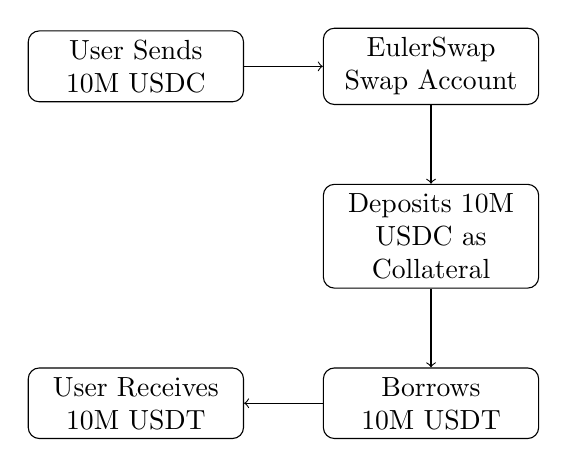
\begin{tikzpicture}[
        node distance=1cm, 
        every node/.style={draw, text width=2.5cm, align=center, rounded corners}
        ]
        % Nodes
        \node (user1) {User Sends 10M USDC};
        \node (EulerSwap) [right=of user1] {EulerSwap Swap Account};
        \node (deposit) [below=of EulerSwap] {Deposits 10M USDC as Collateral};
        \node (borrow) [below=of deposit] {Borrows ~10M USDT};
        \node (user2) [left=of borrow] {User Receives 10M USDT};
        
        % Arrows
        \draw[->] (user1) -- (EulerSwap);
        \draw[->] (EulerSwap) -- (deposit);
        \draw[->] (deposit) -- (borrow);
        \draw[->] (borrow) -- (user2);
    \end{tikzpicture}
    \caption{\textbf{Swap flow in EulerSwap AMM}. EulerSwap’s just-in-time liquidity borrowing. The swap account dynamically increases liquidity by borrowing the ``out token" against the ``in token."}
    \label{fig:EulerSwap_liquidity}
\end{figure}

\section{Virtual reserves and debt limits}

EulerSwap AMMs utilise virtual reserves to simulate larger liquidity pools, effectively increasing the depth of trades that can be serviced. Virtual reserves allow swaps beyond the actual reserves --- the initial collateral deposited by the swap account holder --- by permitting borrowed liquidity, where EulerSwap dynamically loans the out token using the in token as collateral.

Each swap account can configure independent virtual reserve levels. These reserves define the maximum debt exposure an AMM will take on. For instance, if a user deposits \$1,000 in collateral and sets virtual reserves at \$5,000 per vault, the AMM effectively supports up to \$10,000 in combined swap depth, with a loan-to-value (LTV) ratio of 83.3\%. 

Note that the effective LTV must always remain below the borrowing LTV of the lending vault to prevent liquidation. Additionally, different AMM curves influence whether the maximum virtual reserves are achievable.

\subsection{Reserve desynchronisation}

Unlike traditional AMMs, EulerSwap does not hold user funds directly. Instead, it operates as an EVC operator, meaning that all liquidity remains in the wallet of the account holder. This design provides enhanced security and flexibility but introduces the possibility of reserve desynchronisation. Causes of reserve desynchronisation:

\begin{itemize}
    \item \textbf{Interest Accrual:} Over time, collateral deposits earn interest while borrowed tokens accumulate interest costs.
    \item \textbf{External Fund Movements:} A user may manually withdraw funds from a vault, causing EulerSwap’s internal calculations to diverge from actual reserves.
    \item \textbf{Liquidation Events:} If an AMM’s loan-to-value (LTV) ratio exceeds the vault’s risk threshold, automatic liquidation may adjust balances unexpectedly.
\end{itemize}

Users must periodically invoke \texttt{syncVirtualReserves()} to update EulerSwap’s internal state. This function recalculates actual balances and debts relative to the vault and adjusts the virtual reserves accordingly.

\section{Curve}

The space of possible reserves in a EulerSwap AMM is determined by how much debt a swap account is allowed to hold. The EulerSwap curve passes through an equilibrium point $(x_0, y_0)$, at which the marginal price is defined by:

\begin{equation}
\frac{dy}{dx} \Big|_{(x_0, y_0)} = -\frac{p_x}{p_y}.
\end{equation}

Unlike most AMM curves, which are usually defined by a single convex function, EulerSwap uses a piecewise-defined curve, with different functions providing trading behaviour either side of the equilibrium point:

\begin{equation}
    \label{eq:fx-main}
    f(x) =
    \begin{dcases}
        f_1(x), 
        & 0 < x \leq x_0 \\
        f_2(x), 
        & x_0 < x
    \end{dcases}.
\end{equation}

In the domain $0 < x \leq x_0$, the curve is defined by

\begin{equation}
    \label{eq:fx1-main}
    f_1(x) 
    =
    y_{0}+\frac{p_{x}}{p_{y}}\left(x_{0}-x\right)\left(c_{x}+\left(1-c_{x}\right)\left(\frac{x_{0}}{x}\right)\right).
\end{equation}

In the domain $x_0 < x$, the curve is defined by

\begin{equation}
    \label{eq:fx2-main}
    f_2(x) 
    =
    \frac{
        \sqrt{
            \left( \frac{p_x}{p_y} (x - x_0) + y_0 (1 - 2c_y) \right)^2 
            + 4c_y (1 - c_y) y_0^2
        } 
        - \left( \frac{p_x}{p_y} (x - x_0) + y_0 (1 - 2c_y) \right)
    }{2c_y}.
\end{equation}

 The $c_x, c_y$ parameters here are liquidity concentration parameters that control how liquidity is distributed along the curve, with values closer to 1 concentrating liquidity around equilibrium and values closer to 0 distributing it across a wider price range. A full derivation is given in the Appendix \ref{sec:appendix}.  
 
 \begin{figure}[h]  % 'h' places it here, 't' for top, 'b' for bottom, 'p' for separate page
    \centering  % Centers the image
    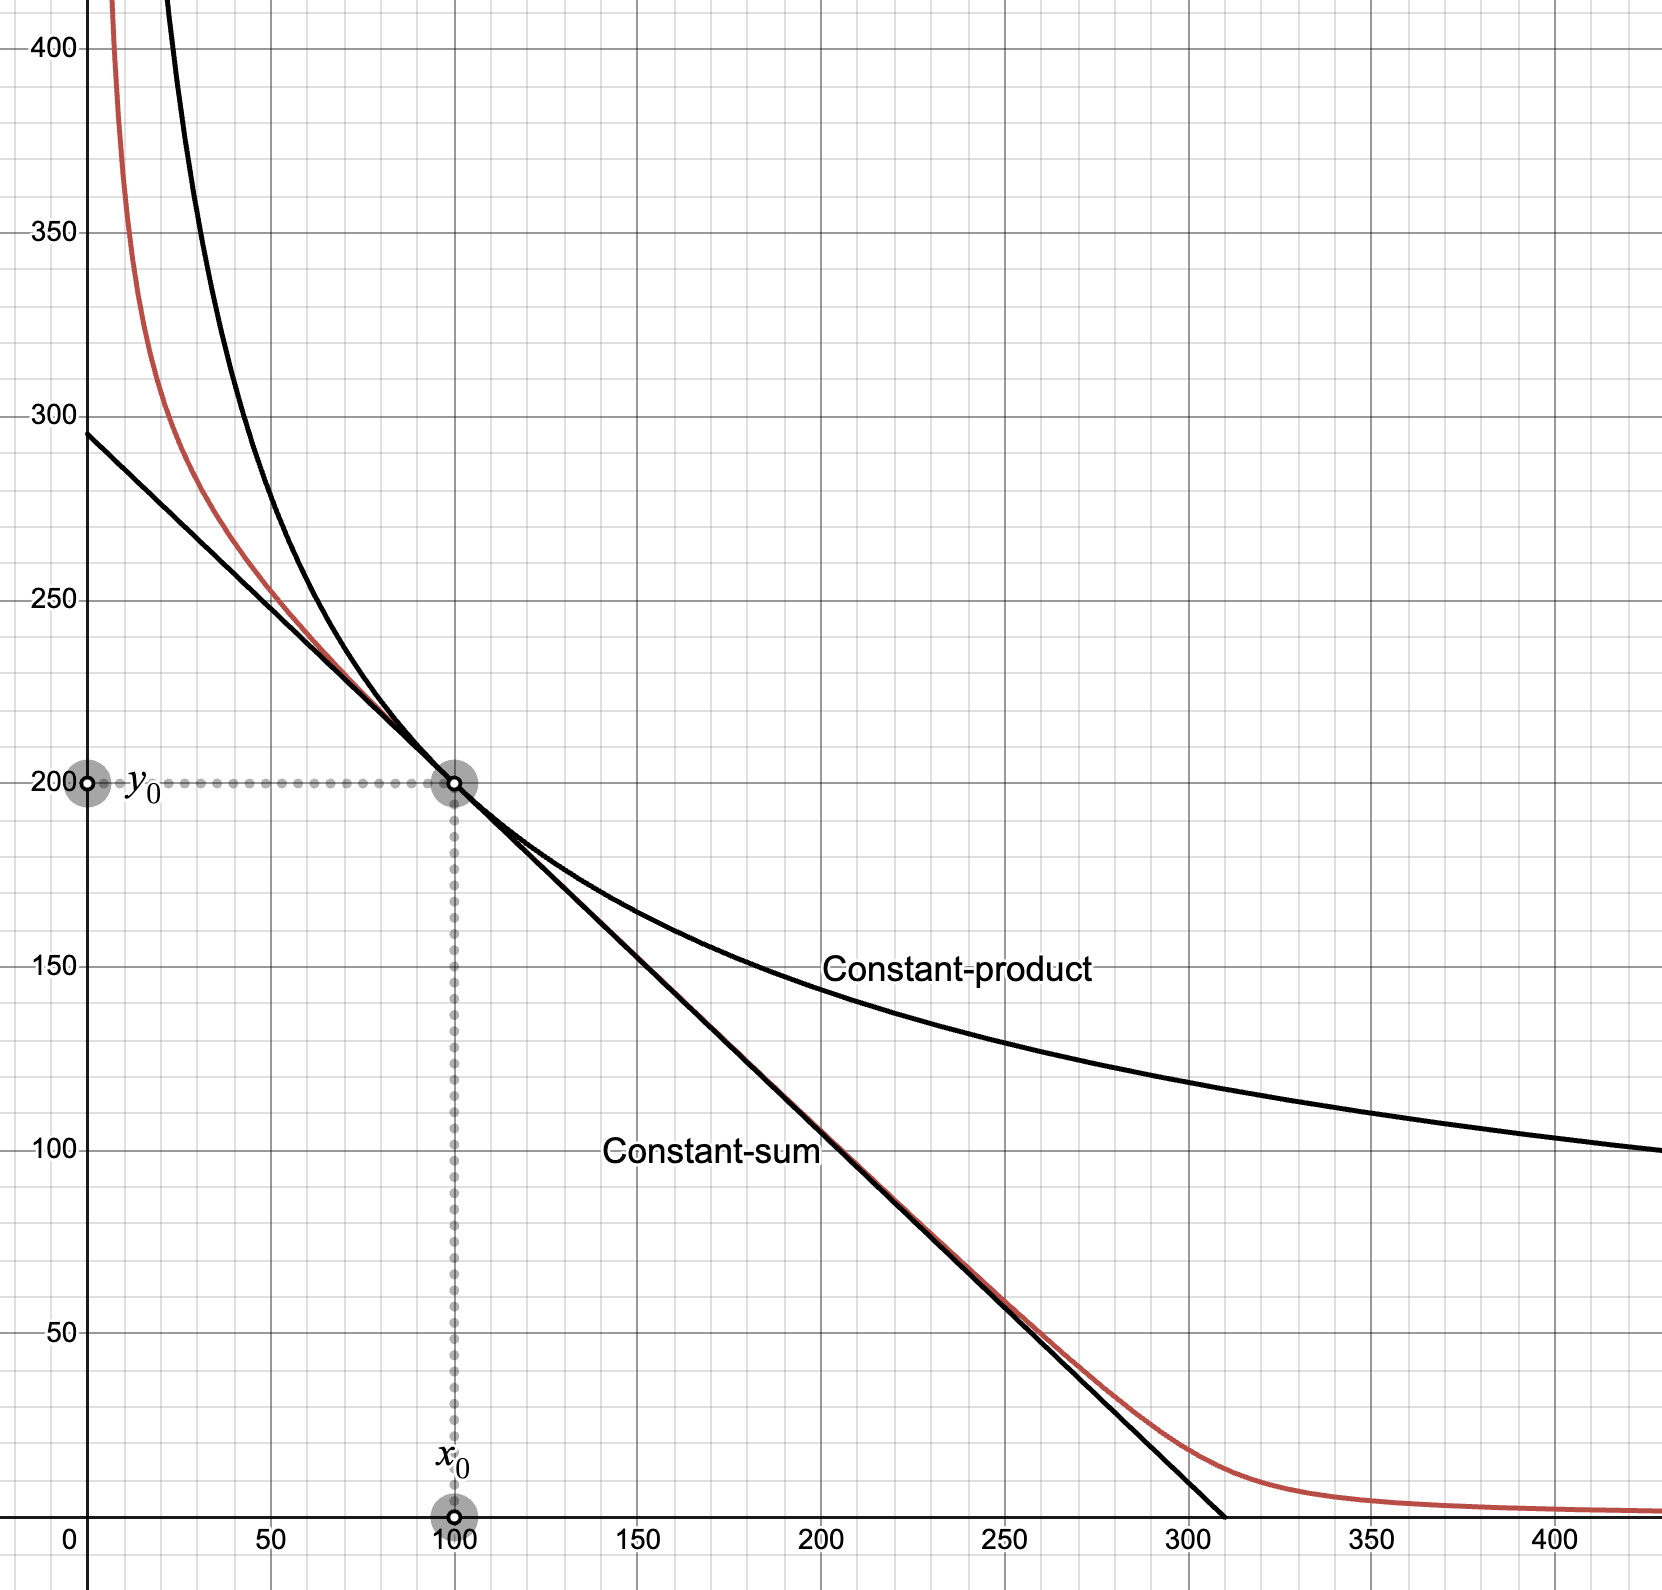
\includegraphics[width=0.5\textwidth]{curve.png} % Adjust width as needed
    \caption{\textbf{EulerSwap AMM curve.} The EulerSwap curve (red line) consists of two sides with separate reserve values $x_0, y_0$ and liquidity concentration parameters $c_x, c_y$, allowing liquidity to be distributed asymmetrically. This means liquidity can be more or less dense or concentrated on one side of the AMM relative to the other. The exchange rate at equilibrium is determined by the pricing parameters $p_x, p_y$ and is fully flexible. You can interact with the curve \href{https://www.desmos.com/calculator/gzwmvbs1dk}{here} on Desmos to compare its behaviour with traditional constant-sum and constant-product curves (black lines).}
    \label{fig:fig1}  % Useful for referencing the figure in text
\end{figure}

\section{Conclusion}

EulerSwap enhances Automated Market Making by leveraging just-in-time borrowing to expand liquidity depth dynamically. By integrating Euler’s lending vaults, it enables market makers to amplify positions efficiently while offering a customisable AMM curve that supports concentrated, distributed, and asymmetric liquidity structures. These features make EulerSwap adaptable to a wide range of trading strategies. However, this efficiency is not without some trade-offs. Swap accounts incur interest costs on borrowed assets, which can erode profitability if not offset by swap fees, interest on collateral, or token incentives. Additionally, EulerSwap inherits Euler’s risk parameters, making it most effective for correlated asset pairs with high loan-to-value (LTV) ratios, while volatile assets pose higher liquidation risks if positions become imbalanced. Despite these trade-offs, EulerSwap represents a breakthrough in AMM design by repurposing idle liquidity in lending protocols, reducing capital inefficiencies, and optimising swap execution. By catering to professional market makers, DAOs, and algorithmic traders, it positions itself as a powerful tool for on-chain liquidity optimisation. Future research could explore optimal strategies for setting liquidity concentration parameters dynamically based on market conditions. EulerSwap's design opens new possibilities for AMM efficiency, setting a foundation for further DeFi innovation.

\section*{Acknowledgments}

During a security review of EulerSwap, Chris Michel noted similarities between some of its underlying concepts and BlackHoleSwap, a project prototype he had reviewed years earlier. While EulerSwap was designed independently and without influence from that project, the resemblance is significant enough to warrant its recognition here as prior art.

\newpage
\section{Appendix}
\label{sec:appendix}

\subsection{Curve derivation}
\label{sec:curve-derivation}

We begin with an Automated Market Maker (AMM) holding initial liquidity reserves of two assets, $X$ and $Y$, denoted as $x_0$ and $y_0$, respectively. In the absence of trading, the AMM remains at equilibrium at the point $(x_0, y_0)$. 

Our goal is to derive a curve for a trading function that supports swaps between the two assets with the following properties:

\begin{itemize}
    \item Passes through the equilibrium point $(x_0, y_0)$.
    \item Maintains an exchange rate, given by the slope of the AMM curve, of $-p_x / p_y$ at $(x_0, y_0)$.
    \item Allows liquidity concentration to be adjusted via parameters $c_x$ and $c_y$, which control the liquidity available for swaps to the left and right of the equilibrium point.
\end{itemize}

To develop such a function, we first introduce two fundamental AMM curve models.

\subsubsection{Constant-sum and constant-product AMM curves}

The constant-sum and constant-product AMM curves are given by:

\begin{align}
    x + y &= x_0 + y_0, \\
    xy &= x_0 y_0.
\end{align}

The constant-sum curve is simply a line, whilst the constant-product curve is a hyperbola. They can be thought of as two extremes when it comes to the distribution of liquidity. The constant-sum curve concentrates liquidity at a single exchange rate, whilst the constant-product curve distributes liquidity across a wide range of different exchange rates. By default, these curves intersect at the point $(x_0, y_0)$, where their slope is:

\[
\frac{dy}{dx} \Big|_{(x_0, y_0)} = -1.
\]

Since real-world markets often operate at variable exchange rates at equilibrium, we introduce custom pricing parameters $p_x$ and $p_y$ to allow flexibility in defining the slope:

\begin{align}
    p_x x + p_y y &= p_x x_0 + p_y y_0, \\
    \label{eq:exponential-form}
    x^{p_y y_0} y^{p_x x_0} &= x_0^{p_y y_0} y_0^{p_x x_0}.
\end{align}

The constant-sum curve is now a line with a slope parameterised by the ratio of the pricing parameters, whilst the constant-product curve is now a weighted hyperbola. Taking the derivatives of these equations with respect to $x$, we obtain:

\begin{align}
    \frac{dy}{dx} &= -\frac{p_x}{p_y}, \\
    \frac{dy}{dx} &= -\frac{p_x}{p_y} \frac{x_0 y}{y_0 x}.
\end{align}

These results confirm that at equilibrium $(x_0, y_0)$, the slope of both functions is:

\[
\frac{dy}{dx} \Big|_{(x_0, y_0)} = -\frac{p_x}{p_y}.
\]

Whilst these curves sufficiently generalise the constant-sum and constant-product curves to an arbitrary price at equilibrium, in practice equation \eqref{eq:exponential-form} has limited practical application as a trading function because it involves an exponential form that is computationally intensive and impractical for on-chain calculations. To resolve this, we introduce the concept of artificial reserves, which simplify price calculations while preserving trading behaviour.


\subsubsection{Introducing artificial reserves for simplicity}

Note that in the interval $0 < x < x_0$ swaps should only increase liquidity beyond $y_0$ and deplete $x_0$ liquidity. That is, our trading function in this interval need not depend on the initial amount of $y_0$ liquidity. This suggests that we can split the domain of the AMM curves into two, and replace the real reserve $y_0$ in the interval $0 < x < x_0$ with an idealised artificial reserve $y_v$. The artificial reserve is chosen such that the value of the reserves, as weighted by their price parameters, are equal at the equilibrium point $(x_0, y_0)$. That is, we have

\[
p_x x_0 = p_y y_v,
\]

such that:

\[
y_v = x_0 \frac{p_x}{p_y}.
\]

Substituting this into our pricing equations for $y_0$ and simplifying, we obtain two modified AMM equations:

\begin{align}
    y &= \frac{p_x}{p_y} (2x_0 - x), \\
    y &= \frac{p_x}{p_y} \frac{x_0^2}{x}.
\end{align}

Since these curves no longer pass through \( (x_0, y_0) \), we correct them by adding back the difference \( y_0 - p_x / p_y x_0 \). This leads to:

\begin{align}
    y &= y_0 + \frac{p_x}{p_y} (x_0 - x), \\
    y &= y_0 + \frac{p_x}{p_y} (x_0 - x) \left( \frac{x_0}{x} \right).
\end{align}

Note that simply shifting the curve up or down like this does not impact the slope or shapes of the curves and therefore has no impact on trading behaviour.

\subsubsection{Unifying into a single curve in the region $0 < x < x_0$}

To create a single unified curve, we introduce a liquidity concentration parameter \( c_x \in [0, 1] \), which determines the curve’s behaviour:

\begin{itemize}
    \item When \( c_x = 1 \), the AMM functions as a constant-sum model.
    \item When \( c_x = 0 \), the AMM behaves as a standard constant-product AMM.
    \item Intermediate values of \( c_x \) create a hybrid liquidity curve.
\end{itemize}

This gives the final equation:

\begin{equation}
    \label{eq:EulerSwap-1}
    y = y_0 + \frac{p_x}{p_y} (x_0 - x) \left( c_x + (1 - c_x) \left(\frac{x_0}{x}\right) \right).
\end{equation}

This is equivalent to the function \( f_1(x) \) given by equation \eqref{eq:fx1-main} in the main text.

\subsubsection{Extending the curve to the \( x > x_0 \) region}

It is important to remember that equation \eqref{eq:EulerSwap-1} only works as a trading function in the interval $0 < x < x_0$. For \( x > x_0 \), we construct a reflected curve that also passes through \( (x_0, y_0) \) and maintains the required derivative:

\begin{equation}
    \label{eq:EulerSwap-3-inverse}
    x = x_0 + \frac{p_y}{p_x} (y_0 - y) \left( c_y + (1 - c_y) \left(\frac{y_0}{y}\right) \right).
\end{equation}

Since this equation defines \( x \) in terms of \( y \), we invert it by solving for \( y \), leading to the quadratic equation:

\begin{equation}
    y = c_y y^2 + \left( \frac{p_x}{p_y} (x - x_0) - y_0(2c_y - 1) \right)y - (1 - c_y) y_0^2.
\end{equation}

Taking only the positive real root, we obtain:

\begin{equation}
    \label{eq:EulerSwap-2}
    y = \frac{
        \sqrt{
            \left( \frac{p_x}{p_y} (x - x_0) + y_0 (1 - 2c_y) \right)^2 
            + 4c_y (1 - c_y) y_0^2
        } 
        - \left( \frac{p_x}{p_y} (x - x_0) + y_0 (1 - 2c_y) \right)
    }{2c_y}.
\end{equation}

This corresponds to the function \( f_2(x) \) given by equation \eqref{eq:fx2-main} in the main text.

\subsection{Invariant derivation}
\label{sec:invariant-derivation}

In traditional AMM protocols, the curve is typically defined as an implicit function of $y$. For example, the classic Uniswap AMM follows a constant-product equation:

\begin{equation}
    xy = x_0 y_0
\end{equation}

where $x_0$ and $y_0$ are the initial liquidity reserves. This equation defines an invariant condition, ensuring that any valid swap must satisfy:

\begin{equation}
    xy \geq x_0 y_0.
\end{equation}

This condition guarantees that after any trade, the product of the new reserves remains at least as large as the initial product, ensuring that swaps cannot drain liquidity from the pool.

Rearranging this condition, we can express the invariant as a lower bound for $y$:

\begin{equation}
    y \geq \frac{x_0 y_0}{x}.
\end{equation}

This means that for any valid trade, the resulting reserve state must lie on or above the AMM curve.  

\subsubsection{Extending the invariant to EulerSwap}

For EulerSwap, we apply a similar principle. Given any reserve state $(x, y)$, we check whether it satisfies an equivalent invariant condition.

From equation \eqref{eq:EulerSwap-1}, for values where \( 0 < x < x_0 \), the AMM curve constraint requires:

\begin{equation}
    \label{eq:invariant-x1}
    y \geq y_{0}+\frac{p_{x}}{p_{y}}\left(x_{0}-x\right)\left(c_{x}+\left(1-c_{x}\right)\left(\frac{x_{0}}{x}\right)\right).
\end{equation}

For values where \( x > x_0 \), we could derive a similar condition for $y$ from equation \eqref{eq:EulerSwap-2}. However, a simpler and computationally cheaper approach is to use the inverse equation \eqref{eq:EulerSwap-3-inverse}, which defines the lower bound for $x$ instead:

\begin{equation}
    \label{eq:invariant-x2}
    x \geq x_{0}+\frac{p_{y}}{p_{x}}\left(y_{0}-y\right)\left(c_{y}+\left(1-c_{y}\right)\left(\frac{y_{0}}{y}\right)\right).
\end{equation}

These conditions together define the valid liquidity states in EulerSwap, ensuring that the AMM remains balanced while allowing for greater flexibility in liquidity provisioning.

\section{Disclaimer}

This paper is for general information purposes only. It does not constitute investment
advice or a recommendation or solicitation to buy or sell any investment and should not
be used in the evaluation of the merits of making any investment decision. It should not
be relied upon for accounting, legal or tax advice or investment recommendations. This
paper reflects current opinions of the authors and is not made on behalf of Euler Labs or its
affiliates and does not necessarily reflect the opinions of Euler Labs, its affiliates or individuals
associated with Euler Labs. The opinions reflected herein are subject to change without being
updated.

\end{document}